\documentclass[12pt,a4paper]{article}
\usepackage[utf8]{inputenc}
\usepackage[english]{babel}
\usepackage{amsmath}
\usepackage{amsfonts}
\usepackage{amssymb}
\usepackage{graphicx}
\usepackage[left=2cm,right=2cm,top=2cm,bottom=2cm]{geometry}
\begin{document}

\raggedright

\section*{Questionnaire 2}

\begin{enumerate}
\item Provide an example of where the bear classification model might work poorly in production, due to structural or style differences in the training data. \\

\smallbreak

There are many cases that the bear classification model could fail, especially if these cases were not represented in the training data:
\begin{itemize}
\item The bear is partially obstructed
\item Nighttime images are passed into the model
\item Low-res images are passed into the model
\item The bear is far away from the camera
\item The bear training dataset is highly biased toward one type of feature (i.e., color)
\end{itemize}

\bigbreak

\item Where do text models currently have a major deficiency? \\

\smallbreak

Text models can generate appropriate text (like replies or imitating author style); however, text models still struggle with generating \textit{correct} responses. Given factual information (such as a knowledge base), it is still hard to generate responses that utilizes this information to generate factually correct responses, though this text can seem very compelling. This can be very dangerous, because people unfamiliar with the subject may not be able to evaluate the factual accuracy of the generated text.

\bigbreak

\item What are possible negative societal implications of text generation models? \\

\smallbreak

The ability for text generation models to generate context-aware, highly compelling responses can be used at a massive scale to spread disinformation and encourage conflict. \\
\smallbreak
Models also reinforce bias (like gender or racial bias) in training data and can create a vicious cycle of biased outputs.

\bigbreak

\item In situations where a model might make mistakes, and those mistakes could be harmful, what is a good alternative to automating a process? \\

\smallbreak

The prediction could then be reviewed by a human professional, who can determine whether the prediction was accurate or not. For example, a machine learning model for identifying strokes in CT scans can alert high priority cases for expedited review, while other cases can be sent to radiologist for regular review. \\
\smallbreak
Other models can also augment a medical professional's abilities, reducing risk but improving efficiency of the workflow. For example, deep learning models can provide useful measurements for radiologists or pathologists.

\bigbreak

\item What kind of tabular data is deep learning particularly good at? \\

\smallbreak

Deep learning is good at analyzing tabular data that includes natural language, or high cardinality categorical items (containing larger number of discrete choices like zip code).

\bigbreak

\item What's a key downside of directly using a deep learning model for recommendation systems? \\

\smallbreak

Current (as of 2020) machine learning approaches for recommendation systems will only tell what products a user might like, and may not be recommendations that would be helpful to the user. For example, if a user if familiar with other books from the same author, it isn't helpful to recommend those products even though the user bought the author's book. 

\bigbreak

\item What are the steps of the Drivetrain Approach? \\

\smallbreak

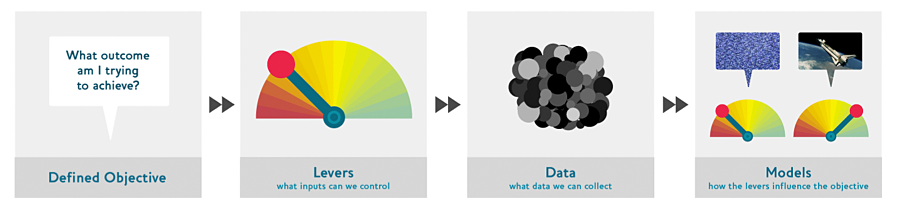
\includegraphics[scale=0.5]{drivetrain.png}

\bigbreak

\item How do the steps of the Drivetrain Approach map to a recommendation system? \\

\smallbreak

The \textbf{objective} of a recommendation engine is to drive additional sales by surprising and delighting the customer with recommendations of items they would not have purchased without the recommendation. The \textbf{lever} is the ranking of the recommendations. New \textbf{data} must be collected to generate recommendations that will cause new sales . This will require conducting many randomized experiments in order to collect data about a wide range of recommendations for a wide range of customers. This is a step that few organizations take; but without it, you don’t have the information you need to actually optimize recommendations based on your true objective (more sales!)

\bigbreak

\item Create an image recognition model using data you curate, and deploy it on the web. \\

Placeholder

\item What is \verb/DataLoaders/? \\

\smallbreak

The \verb/DataLoaders/ class is the class that passes the data to the fastai model. It is essentially a class that stores the required \verb/DataLoader/ objects (usually for train and validation sets).

\bigbreak

\item What four things do we need to tell fastai to create \verb/DataLoaders/? \\

\smallbreak

\begin{itemize}
\item what kinds of data we are working with
\item how to get the list of items
\item how to label these items
\item how to create the validation set
\end{itemize}

\bigbreak

\item What does the splitter parameter to \verb/DataBlock/ do? \\

\smallbreak

The splitter parameter is used as a way for fastai to split up the dataset into multiple subsets (usually train and validation sets). For example, to randomly split the data, you can use fastai's predefined \verb/RandomSplitter/ class, providing it with the proportion of the data used for validation.

\bigbreak

\item How do we ensure a random split always gives the same validation set? \\

\smallbreak

It turns out that it is impossible to create truly random numbers. Instead, computers use a process known as a pseudo-random generator. However, this process can be controlled using a random seed. By setting a seed value, the pseudo-random generator will generate the same "random" numbers in a fixed manner which will be the same for every run as long as the seed is the same. By using a random seed, we can generate a random split that always gives the same validation set.

\bigbreak

\item What letters are often used to signify the independent and dependent variables? \\

\smallbreak


\item What's the difference between the crop, pad, and squish resize approaches? When might you choose one over the others? \\
\item What is data augmentation? Why is it needed? \\
\item What is the difference between item\_tfms and batch\_tfms? \\
\item What is a confusion matrix? \\
\item What does export save? \\
\item What is it called when we use a model for getting predictions, instead of training? \\
\item What are IPython widgets? \\
\item When might you want to use CPU for deployment? When might GPU be better? \\
\item What are the downsides of deploying your app to a server, instead of to a client (or edge) device such as a phone or PC? \\
\item What are three examples of problems that could occur when rolling out a bear warning system in practice? \\
\item What is "out-of-domain data"? \\
\item What is "domain shift"? \\
\item What are the three steps in the deployment process? \\
\end{enumerate}

\section*{Further Research}

\begin{enumerate}
\item Consider how the Drivetrain Approach maps to a project or problem you're interested in. \\
\item When might it be best to avoid certain types of data augmentation? \\
\item For a project you're interested in applying deep learning to, consider the thought experiment "What would happen if it went really, really well?" \\
\item Start a blog, and write your first blog post. For instance, write about what you think deep learning might be useful for in a domain you're interested in. \\
\end{enumerate}

\end{document}